\documentclass[10pt,a4paper]{article}
\usepackage[utf8]{inputenc}
\usepackage[english]{babel}
\usepackage[T1]{fontenc}
\usepackage{amsmath}
\usepackage{amsfonts}
\usepackage{amssymb}
\usepackage{makeidx}
\usepackage{graphicx}
\usepackage{fourier}
\usepackage{listings}
\usepackage{color}
\usepackage{hyperref}
\usepackage[left=2cm,right=2cm,top=2cm,bottom=2cm]{geometry}
\author{Johannes Scheller (candidate no. 71), Vincent Noculak\\ Lukas Powalla (candidate no. 67), Richard Asbah}
\title{Computational Physics - Project 4}

\lstset{language=C++,
	keywordstyle=\bfseries\color{blue},
	commentstyle=\itshape\color{red},
	stringstyle=\color{green},
	identifierstyle=\bfseries,
	frame=single}
\begin{document}

\maketitle
\newpage
\tableofcontents
\newpage

\section*{Introduction}
In project 4 we are dealing with the Ising model in two dimensions without an external magnetic field. We are looking at a lattice of L times L particles, where each particle has a spin value of $\pm 1$. In order to compute different interesting properties of the system, we want to use the metropolis algorithm.  With our computations, we want to calculate the Energy, the absolute value of the magnetisation, the heat capacity and susceptibility of the system as a function of temperature in order to study phase transitions of the system. 
In our case, we want to study the phase transition from a ordered phase for low temperatures to a disordered phase for high temperatures above the critical Temperature $T_c$(in a canonical ensemble this means a second order phase transition and therefore a divergence of the heat capacity at the critical Temperature).
In order to get familiar with all the quantities, we first wan to study the case of a 2 times 2 lattice. For This lattice-size, we want to find a analytical expression for all interesting physical properties of the system and compare them with the computed values.
However, researcher have solved the two dimensional Ising model a long time ago for any and even for infinite size.
The Ising model in two dimensions has been solved first for any "fixed" size by Kaufman in 1949 and in the end even for a infinite size by Onsager in 1944.  (compare with "Statistical Mechanics: Algorithms and Computations; Werner Krauth; published 2006")
This project may also show the link from statistical physics to macroscopic properties of a given physical system, which is a interesting relation.
\section{Theory}

\subsection{General properties of physical systems and their link to statistical physics}

\subsubsection{physical ensembles}
%Lukas changed this; newest version 08.11.15
Let us now look at a physical system and its surroundings. 
In principle, it is necessary to describe the relation of the physical system and its surroundings in order to determine the properties of the system.(sometimes this relations are related to physical boundary conditions) It is necessary to know whether we want to allow for instance particle/heat exchange or not. How we set up our system also defines us the thermodynamic potential, which can be used to describe the system.(e.g. Entropy, Helmholtz,Gibbs) All in all, we have the Microcanonical ensemble, the canonical ensemble, the Grandcanonical ensemble and the pressure canonical ensemble. (in this case an ensemble means a collection of mircoscopic systems, compare with the lecture notes Computational physics 2015 at University of Oslo by Morten Hjorth-Jensen page 417 )
In the following, we will always deal with the canonical ensemble. This  means that we don't allow particle exchange from the system with its surroundings, but we allow exchange of heat with the environment. 
Fixed variables are in this case the temperature, the total volume and the total particle number. The total energy of the canonical ensemble is not constant, because there can be heat exchange with the surroundings. The system, which does not allow heat exchange and does not allow particle exchange is called micro-canonical ensemble. (compare "Statistical Mechanics  An Intermediate Course; 2nd Edition; G. Morandi/F. Napoli/ E. Ercolessi; page 94ff") 


\subsubsection{General properties of canonical ensembles}\label{General properties of canonical ensembles}
%Lukas changed this; newest version 08.11.15
The canonical ensemble can be expressed by Helmholtz' free energy. The system strives to a minimum of Helmholtz' free energy, which is defined as follows:
\begin{equation}
F=-k_BTlnZ = <E>-TS \label{F}
\end{equation}
where the entropy S is given by
\begin{equation}
S=-k_BlnZ + k_B T \frac{\partial lnZ}{\partial T}\label{S}
\end{equation}
We can see that $F$ depends on the expectation value of the Energy and on $-TS$. 
Hence, the canonical ensemble pursuits towards an energy minimum and higher entropy. This can be interpreted as a "struggle between two important principles in physics"( lecture notes Computational physics 2015 at University of Oslo by Morten Hjorth-Jensen page 419 )
The probability distribution for a canonical ensemble is given by the Boltzmann distribution.

\begin{align}
P_i (\beta) =\frac{ e^{- \beta E_i}}{Z}
\end{align} 
$\beta = 1/k_B T$ where T is the temperature, $k_B$ is the Boltzmann constant,$E_i$ is the energy of micro state i and Z is the partition function for the canonical ensemble is the sum over all the micro states M.

\begin{equation}
  Z=\sum_{i=1}^{M}e^{- \beta E_i}
\end{equation}
   
After running the system for long time the canonical ensemble is uniquely determined and does not depend on the arbitrary choices of the initial temperature.
The system uncertainty due the Energy fluctuations in the canonical ensemble gives the variance of the energy.\\
 
%from here on,  Richards actual part


\centerline{ from equation \ref{F}, \ref{S} and probability distribution $P_i$ }
\begin{align}
<E> = k_b T^2 \frac{\partial lnZ}{\partial T}=\sum_{i=1}^{M} E_iP_i(\beta)=\frac{1}{Z }\sum_{i=1}^{M}E_i e ^{ - \beta E_i}
\end{align}
The heat capacity is how much the energy change due to the change in the temperature. The heat capacity $C_V$ can be defined as

\begin{equation}
C_V =\frac{\partial E}{\partial T} 
\end{equation}

\begin{equation}
\frac{\partial}{\partial T}\frac{1}{Z} = \frac{\partial}{\partial T}\frac{1}{\sum_{i=1}^{M}e^{- \frac{1}{k_BT} E_i}} = -\frac{1}{k_B T^2 } \frac{\sum_{i=1}^{M} E_i e^{-E_i \frac{1}{k_BT}}}{\left(\sum_{i=1}^{M} e^{-E_i \frac{1}{k_BT}} \right)^2}=-\frac{1}{k_B T^2 } \frac{\sum_{i=1}^{M} E_i e^{-E_i \frac{1}{k_BT}}}{\left( Z\right)^2}
\end{equation}

\begin{equation}
\frac{\partial}{\partial T}\sum_{i=1}^{M}E_i e ^{ - \frac {1}{k_BT} E_i} = \frac{1}{k_BT^2}\sum_{i=1}^{M}E_i^2 e ^{ - \frac {1}{k_BT} E_i}
\end{equation}

\begin{align}
C_V &=\frac{\partial <E>}{\partial T} = \frac{\partial}{\partial T} \left( \frac{1}{Z }\sum_{i=1}^{M}E_i e ^{ - \frac {1}{k_BT} E_i}\right) = -\frac{1}{k_B T^2 } \frac{\sum_{i=1}^{M} E_i e^{-E_i \frac{1}{k_BT}}}{ Z^2}\sum_{i=1}^{M}E_i e ^{ - \frac {1}{k_BT} E_i} +\frac{1}{Z}\frac{1}{k_BT^2}\sum_{i=1}^{M}E_i^2 e ^{ - \frac {1}{k_BT} E_i} \\
 &= -\frac{1}{k_B T^2 } \left( \frac{\sum_{i=1}^{M} E_i e^{-E_i \frac{1}{k_BT}}}{ Z} \right)^2 +\frac{1}{Z}\frac{1}{k_BT^2}\sum_{i=1}^{M}E_i^2 e ^{ - \frac {1}{k_BT} E_i} = \frac{1}{k_B T^2 } \left( <E>^2 - <E^2> \right)
\end{align}
The magnetic susceptibility is a measurable quantity, which indicates if the material is attracted or repelled of a magnetic field.
Magnetic materials can be classified as paramagnetic, diamagnetic or ferromagnetic based on their susceptibility.

\begin{equation}
\chi =\frac{\partial <M>}{\partial H} 
\end{equation}
We can evaluate the mean magnetization through:

\begin{equation}
<M> = \sum_{i}^{M}M_iP_i(\beta)= \frac{1}{Z}\sum_{i}^{M}M_ie^{- \frac{E_i}{k_BT}}
\end{equation}
The total energy of the system in addition of external magnetic field H can be described with:

\begin{equation}
E = -\sum_{i,j} J_{s_is_j}- H\sum_{i}s_i
\end{equation}
The magnetization is the sum of all spin for a given configuration:
\begin{equation}
\frac{\partial E_i}{\partial H} =- \sum_{i}s_i = -M_i
\end{equation}

\begin{equation}
\frac{\partial}{\partial H}\frac{1}{Z} = \frac{\partial}{\partial H}\frac{1}{\sum_{i=1}^{M}e^{- \frac{1}{k_BT} E_i}} = -\frac{1}{k_B T} \frac{\sum_{i=1}^{M} M_i e^{-E_i \frac{1}{k_BT}}}{\left(\sum_{i=1}^{M} e^{-E_i \frac{1}{k_BT}} \right)^2}=-\frac{1}{k_B T} \frac{\sum_{i=1}^{M} M_i e^{-E_i \frac{1}{k_BT}}}{\left( Z\right)^2}
\end{equation}

\begin{equation}
\frac{\partial}{\partial H}\sum_{i=1}^{M}M_i e ^{ - \frac {1}{k_BT} E_i} = \frac{1}{k_BT}\sum_{i=1}^{M}M_i^2 e ^{ - \frac {1}{k_BT} E_i}
\end{equation}

\begin{align}
\chi &=\frac{\partial <M>}{\partial H} = \frac{\partial}{\partial H} \left( \frac{1}{Z }\sum_{i=1}^{M}M_i e ^{ - \frac {1}{k_BT} E_i}\right) = -\frac{1}{k_B T } \frac{\sum_{i=1}^{M} M_i e^{-E_i \frac{1}{k_BT}}}{ Z^2}\sum_{i=1}^{M}M_i e ^{ - \frac {1}{k_BT} E_i} +\frac{1}{Z}\frac{1}{k_BT}\sum_{i=1}^{M}M_i^2 e ^{ - \frac {1}{k_BT} E_i} \\
 &= -\frac{1}{k_B T} \left( \frac{\sum_{i=1}^{M} M_i e^{-E_i \frac{1}{k_BT}}}{ Z} \right)^2 +\frac{1}{Z}\frac{1}{k_BT}\sum_{i=1}^{M}M_i^2 e ^{ - \frac {1}{k_BT} E_i} = \frac{1}{k_B T } \left( <M>^2 - <M^2> \right)
\end{align}


\subsubsection{Ferromagnetic order}
% not clearly understandeble (comment by Lukas )
A ferromagnet has a spontaneous magnetic moment even with the absence of an external magnetic field. Due the existence of a spontaneous moment the electron spin and magnetic moments must be arranged in a regular manner.
In a ferromagnet most of the spins are aligned and in an  anti ferromagnet the most of neighbouring spins are pointing in opposite directions.
(compare "Introduction to Solid States Physics- 8th edition, by Charles kittel, page 323)
In general -in a ferromagnet- spins up want to be next to spin up and spin downs want to be next to spin downs. At low temperature, the spin system is magnetised (either mostly up or mostly down). However, at high temperatures above the critical temperature, up and down spins are equally likely and the spins will in total cancel each other out. (total magnetisations is zero)

\subsubsection{link from the Macroscopic values to statistical physics}
%Lukas newest upgrade 08.11.15
In chapter \ref{General properties of canonical ensembles}, we derived the expression of the heat capacity and of the magnetic susceptibility of a canonical ensemble. We didn't care about statistical properties. However, what strikes the eye is that in the expression of the heat capacity as well as in the expression of the magnetic susceptibility, we see that they both depend on the variance of the energy of the magnetisation. this means that they can be written as:
\begin{align}
C_v &= \frac{1}{k_B T^2}\cdot \mathrm{Var(E)}\\
\chi &= \frac{1}{k_B T} \cdot \mathrm{Var(M)}
\end{align}
The variance measures how far away a set of numbers is spread out. A huge variance means then that the values of the quantity fluctuate a lot around the expectation value.  Now, we have linked a statistical property to a thermodynamic and macroscopic such as heat capacity. 
\subsection{theoretical numerical solutions}

\subsubsection{Ising model}
Ising model is a mathematical model for ferromagnetism studies of phase transitions for magnetic system at given a temperature. The model consists the interaction between two neighbouring spins is related by the interaction energy 
\begin{equation}
  -Js_ks_l
\end{equation} 
where the sin s can be in two states +1 or -1,where  $s_k$ and $s_l$ are the nearest neighbors. Which give a low energy (-J) if the two spin aligned and high energy (j) for spin pointing in opposite direction. The total energy to a system with N number of spins and with the absence of magnetic field can be expressed as 
\begin{equation}
  E=-J\sum_{<kl>}^{N}s_ks_l
\end{equation}

  
  \subsubsection{Periodic boundary conditions} 
Periodic boundary conditions is used for approximating a large or infinite system by using smaller repeating system, we will impose PBCs on our spin lattice in x and y directions.

 s(L+1,y) = s(1,y)
 
 s(x,L+1) = s(X,1)  


\subsubsection{Metropolis algorithm in the two dimensional Ising model}
The Ising model with Metropolis algorithm generates a sequence of states with Monte Carlo path, where the transition between states depends on the transition probability between the next and current state. The probability distribution is given by the Boltzmann distribution which is the probability for finding the system in a state s.
\begin{align}
Ps =\frac{ e^{- \beta E_i}}{\sum_{i=1}^{M}e^{- \beta E_i}}
\end{align}
It is difficult to compute since we need the sum over all states. If we have a 10 x 10 spin lattice interacting in our Ising model, there are $2^{100}$ possible states. Computing the sum seems to be not that efficient, but luckily the Metropolis algorithm needs only the ratios between the state probabilities and we do not need to compute the sum of all the states after all. The Metropolis algorithm in this case can be implement by establishing two dimensional Ising model with random lattice configuration. Then we flip a randomly chosen spin and compute the energy difference $\Delta E$. If $\Delta E \leq 0$ we accept the flip, otherwise we compute the transition probability $w = e^-{\beta \Delta E}$ and compare with a random number r.\\If $r \leq w$ we accept the flip otherwise we keep the old configuration. We can keep choosing new random spins until we are satisfied with a good representation of the states.(compare to"lecture notes Computational physics 2015 at University of Oslo by Morten Hjorth-Jensen page 435)"   


\subsubsection{Critical temperature (Lars Onsager)}
in 1944 the Norwegian chemist Lars Onsager made very important discovery in theoretical physics, namely the exact solution of the Ising spin model in two dimensions. His work is up to now a valid theoretical description of the two dimensional Ising model. Onsager's solutions achieved the thermodynamic properties of interaction systems and phase transitions at $T_c$. However in 1942 Lars Onsager solved the two dimensional model for zero field energy, which has been published two years after. In 1948, he wrote the solution for the zero field magnetization in a conference at Cornell. Onsager showed how to derive the partition function for the canonical ensemble with zero external magnetic field Z(B = 0,T)with N spins.
\begin{align}
 Z_N =  \left( 2 \mathrm{cosh}(\beta J)e^{I} \right)^N 
\end{align}
where $ I = \frac{1}{2\pi} \int_{0}^{\pi} d \phi ln \bigg[ \frac{1}{2} \left( 1 + \sqrt{1-\kappa^2 \mathrm{sin} ^2 \phi} \right) \bigg]$
where $\kappa = \frac {2\mathrm{sinh}(2\beta J)}{\mathrm{cosh}^2(2\beta J)}$
and the energy is given by
\begin{align}
 <E> = -J\mathrm{coth}(2\beta J) \bigg[ 1+\frac{2}{\pi}(2\mathrm{tanh}^2(2\beta J)-1)K_1(q) \bigg] 
\end{align}
where $q = \mathrm{sinh}(2\beta J)/\mathrm{cosh}^2(2\beta J)$ and the complete elliptic integral of the first kind is:
\begin{align}
k_1(q) = \int_{0}^{\frac{\pi}{2}} \frac{d\phi}{\sqrt{1-q^2\mathrm{sin}^2 \phi}} 
\end{align}
and differentiating the energy with the respect to temperature we obtain the specific heat:

\begin{align}
C_v = \frac{\partial <E>}{\partial T} = \frac{4K_B}{\pi}(\beta J \mathrm{coth}(2\beta J) )^2 \bigg\{ K_1(q)-K_2(q)-(1-\mathrm{tanh}^2(2\beta J))\bigg[ \frac{\pi}{2}+(2\mathrm{tanh}^2(2\beta J)-1 )K_1(q) \bigg] \bigg\}
\end{align}
where 
\begin{align}
k_2(q) = \int_{0}^{\frac{\pi}{2}} d \phi \sqrt{1-q^2\mathrm{sin}^2\phi}
\end{align}
Near the critical temperature $T_c$ the specific heat behaves as:
\begin{align}
C_v \approx -\frac{2}{\pi}\left( (\frac{2J}{K_BT_c}\right)^2 ln \Bigg[ 1- \frac{T}{T_c}\Bigg]+ const.
\end{align}

\begin{align}
C_v \sim \Bigg| 1- \frac{T}{T_c}\Bigg|^{\alpha}
\end{align}
the limiting form of the function
\begin{align}
\lim_{\alpha \to 0} \frac{1}{\alpha}(\mathrm{Y}^{-\alpha}-1)=-ln\mathrm{Y}
\end{align}
can be used to infer that closed-form result in low singularity with $\alpha = 0.$
We do not want t make a complete derivation of Onsager's result, however we want to limit ourselves to his final result for the expectation value of the magnetisation:

\begin{align}
<\frac{M(T)}{N}> = \Bigg[ 1- \frac{(1 - \mathrm{tanh} ^2(\beta J))^{4}}{16\mathrm{tanh}^{4}(\beta J)} \Bigg] ^{\frac{1}{8}} \label{Onsager magnetisation}
\end{align}
for $T<T_c.$ otherwise the magnetization is zero 
"lecture notes Computational physics 2015 at University of Oslo by Morten Hjorth-Jensen page 435)" 


From Onsager's result, we get <M(t)/N>. $T_c$ is the temperature, where we start getting a non zero magnetization. When we heat up the system, we start with non-zero magnetisation until we pas the critical Temperature. From there on, we have zero magnetisation.
If we want now to calculate the critical Temperature, we can set the equation \ref{Onsager magnetisation} to zero. The temperature belonging to this is the critical temperature:
   
\begin{align}
<M(T)/N> = \Bigg[ 1- \frac{(1 - \mathrm{tanh} ^2(\beta J))^{4}}{16\mathrm{tanh}^{4}(\beta J)} \Bigg] ^{\frac{1}{8}} = 0
\end{align}

the only way to obtain <M>=0 is when equation \ref{critical temperature derivation} is valid. 
\begin{align}
\frac{(1 - \mathrm{tanh}^2(\beta J))^{4}}{16\mathrm{tanh}^{4}(\beta J)} = 1 \label{critical temperature derivation}
\end{align}
This gives us:
\begin{align}
0&=\mathrm{tanh}(\beta J )^2+2 \cdot \mathrm{tanh}(\beta J ) -1 \\
\mathrm{tanh}(J \beta ) &= \frac{-2 \pm \sqrt{4+4}}{2} = -1 \pm \sqrt{2}\\
\beta J &= \mathrm{arctanh}(-1 \pm \sqrt{2})\\
&= \frac{1}{2} ln(1+\sqrt{2})\\
\Rightarrow \frac {k_B T_c}{J} &= \frac{2}{ln(1+\sqrt{2})}\approx 2.2692
\end{align}
Now, we found the critical temperature of 2.2692 (dimensionless unit)
Near the critical temperature, we can describe the behaviour of the different quantities through the so called "power law". However, we want not dive deeper into this topic and name just specific results, which can be derived with this method.
\begin{align}
<M(T)> & \propto (T-T_c)^{\frac{1}{8}}\\
C_v & \propto \left| T_c - T \right|^{\alpha}\\
\chi ( t)& \propto \left| T_c - T \right|^{\gamma}\\
\end{align}
with $\alpha=0, \gamma=\frac{7}{4} $. In addition to that, we can describe the correlation length of the system by $\xi(T) $:
\begin{align}
\xi (T) \propto \left| T_c - T \right|^{-\nu}
\end{align}

\subsection{Closed solution for a 2 dimensional 2 x 2 lattice \label{closed_solution}}

We want now to look at a 2 x 2 lattice and we want to calculate the partition function, the energy, magnetisation, heat capacity and susceptibility of the system  dependent of T. 
The partition function for a canonical ensemble with periodic boundary conditions can be computed  by:
\begin{align}
Z= \sum_{i=1}^{M} e^{- \beta E_i}
\end{align} 
Here, $\beta$ is $\frac{1}{k_b \cdot T}$, where $k_b$ is the Bolzmann constant. 
In this expression we sum over all microstates m. The Energy of the system in configuration i is then:
\begin{align}
E_i = - J \sum_{<kl>}^N s_k s_l 
\end{align} 

The sum over $<kl>$ means that we only sum over nearest neighbours. In our 2 x 2 case, we have for each "particle" two possible values $\pm 1$. This means that we have all in all $2^{2 \cdot 2} = 2^4=16$ micro states. We have to compute the Energy of the micro states in order to compute the partition function. 
We also want to introduce the magnetisation, which is simply the sum over all the spins of the system:
\begin{align}
M_i=\sum_{j=1}^N s_j
\end{align}
We want also to introduce the so called degeneracy, which counts the number of micro states for a given micro energy. We get the following table:
\begin{figure}[h]
\centering
\caption{Energy of the different micro states}
\label{table of microstates}
\begin{tabular}{c|c|c|c}
Number of spins up (+1) & Degeneracy &  Energy & Magnetization\\
\hline \hline
4 & 1 & $-8J$ & 4 \\
3 & 4 & 0 & 2 \\
2 & 4 & 0 & 0 \\
2 & 2 & $8J$ & 0 \\
1 & 4 & 0 & -2 \\
0 & 1 & $-8J$ & -4 
\end{tabular}
\end{figure}
We can now write the expression of the partition function as in equation \ref{Partition 2x2}. We used the Table \ref{table of microstates} to calculate the sum over the micro states. 
\begin{align}
Z&= \sum_{i=1}^{M} e^{- \beta E_i}= 12 \cdot e^{-\beta \cdot 0 } + 2 \cdot e^{-8J \beta } + 1 \cdot e^{8J \beta } + 1 \cdot e^{8J \beta } \\
&= 12+ 2 \cdot e^{-8J \beta } + 2 \cdot e^{8J \beta } \\
&= 12+ 4 \cdot \mathrm{cosh} \left( 8J \beta \right) \label{Partition 2x2}
\end{align} 
We can now calculate the expectation value of the energy. There are two possible ways of calculating it. the first way of calculating the expectation value of the energy can be seen in equation \ref{Energyexpectation way1}. 
\begin{align}
<E>&= - \frac{\partial ln(Z)}{\partial \beta} =-\frac{1}{Z} \cdot 32J  \cdot \mathrm{sinh}(8J \beta ) \\ \label{Energyexpectation way1}
&= -\frac{32 J \cdot \mathrm{sinh}((8J \beta )}{Z}\\
&=-\frac{8 \cdot J \cdot  \mathrm{sinh}(8J \beta ) }{3+\mathrm{cosh}(8J\beta)}
\end{align}
Alternatively, we can calculate the expectation value of the Energy by looking at the micro states:
\begin{align}
<E> = \frac{1}{Z} \sum_{i=1}^{M} E_i e^{- \beta E_i}=-\frac{8 \cdot J \cdot  \mathrm{sinh}(8J \beta ) }{3+\mathrm{cosh}(8J\beta)}
\end{align}
Both expressions are equal. Next, we want to determine the expectation value of the magnetisation. We use the formula \ref{expectation magnetisation 2x2}. We can see that we get 0 for the expectation value of the magnetisation. 
\begin{align}
<M> &= \frac{1}{Z} \sum_{i}^M M_i \cdot e^{- \beta E_i }\\\label{expectation magnetisation 2x2}
&= \frac{1}{Z} \cdot \left( 4 \cdot 1 \cdot e^{-8J\beta}+ 2 \cdot 4+(-2) \cdot 4 + (-4) \cdot 1 \cdot e^{-8J \beta } \right)\\
&=0
\end{align}
However, we are interested in the expectation value of the absolute value of magnetisation, which is $<|M|>$. This expression can be determined as follows:
\begin{align}
<|M|> &= \frac{1}{Z} \sum_{i}^M |M_i| \cdot e^{- \beta E_i }\\\label{expectation absolute magnetisation 2x2}
&= \frac{1}{Z} \cdot \left( |4| \cdot 1 \cdot e^{8J\beta}+ |2| \cdot 4+|(-2)| \cdot 4 + |(-4)| \cdot 1 \cdot e^{8J \beta } \right)\\
&=\frac{1}{Z} \cdot \left( 8 \cdot e^{8J\beta} +16 \right)\\
&= \frac{2 \cdot e^{8J\beta}+4}{3+ \mathrm{cosh}(8J\beta)}
\end{align}
In order to describe how the temperature will change when thermal energy is added to the system, we want to look at a quantity called heap capacity. ($C_v$) The bigger this quantity is the less heats the system up by a given amount of thermal energy, which is added to the system.  
\begin{align}
C_v &= \frac{1}{k_b T^2} \left( \frac{1}{Z} \sum_{i=1}^{M} E_i^2 e^{- \beta E_i } - \left( \frac{1}{Z} \sum_{i=1}^{M} E_i e^{- \beta E_i }  \right)^2 \right)\\
&=\frac{1}{k_b T^2} \left( \frac{1}{Z} \left( 2 \cdot (8J)^2 \cdot e^{8J \beta}+2 \cdot (-8J)^2 \cdot e^{-8J \beta} \right) - \left( \frac{8 \cdot J \cdot  \mathrm{sinh}(8J \beta ) }{3+\mathrm{cosh}(8J\beta)} \right)^2 \right)\\
&=\frac{1}{k_b T^2} \left( \frac{64\cdot J\cdot \mathrm{cosh}(8 J \beta )}{3+\mathrm{cosh}(8J\beta)}  - \left( \frac{8 \cdot J \cdot \mathrm{sinh}(8J \beta ) }{3+\mathrm{cosh}(8J\beta)} \right)^2 \right)\\
&= \frac{1}{k_b T^2} \left( \frac{64 \cdot J +3\cdot J \cdot 64 \mathrm{cosh}(8J \beta)}{\left(3+\mathrm{cosh}(8J\beta)\right)^2} \right)\\
&= \frac{64}{k_b T^2} \left( \frac{ J +3 J \cdot \mathrm{cosh}(8J \beta)}{\left(3+\mathrm{cosh}(8J\beta)\right)^2} \right)\\
\end{align}
At last, we want to have a look at the magnetic susceptibility. This quantity is a magnetic property of the material. The magnetic susceptibility describes the response of the material to an applied magnetic field. 
\begin{align}
\chi &= \frac{1}{k_b T} \cdot \left( \frac{1}{Z} \sum_{i=1}^{M} M_i^2 e^{- \beta E_i } - \left( \frac{1}{Z} \sum_{i=1}^{M} M_i e^{- \beta E_i }  \right)^2 \right)\\
&= \frac{1}{k_b T} \cdot \left( \frac{1}{Z} \cdot \left( 4^2 \cdot 1 \cdot e^{8J\beta}+ 2^2 \cdot 4+(-2)^2 \cdot 4 + (-4)^2 \cdot 1 \cdot e^{8J \beta } \right) - \left( 0  \right)^2 \right)\\
&= \frac{1}{k_b T} \cdot \frac{32 e^{8J\beta}+32}{ 12+ 4 \cdot \mathrm{cosh} \left( 8J \beta \right)}\\
&= \frac{1}{k_b T} \cdot \frac{8 e^{8J\beta}+8}{ 3+ \cdot \mathrm{cosh} \left( 8J \beta \right)}\\
\end{align}

\begin{align}
\chi_{abs} &= \frac{1}{k_b T} \cdot \left( \frac{1}{Z} \sum_{i=1}^{M} M_i^2 e^{- \beta E_i } - \left( \frac{1}{Z} \sum_{i=1}^{M} |M_i| e^{- \beta E_i }  \right)^2 \right)\\
&= \frac{1}{k_b T} \cdot \left( \frac{1}{Z} \cdot \left( 4^2 \cdot 1 \cdot e^{8J\beta}+ 2^2 \cdot 4+(-2)^2 \cdot 4 + (-4)^2 \cdot 1 \cdot e^{8J \beta } \right) - \left( \frac{2 \cdot e^{8J\beta}+4}{3+ \mathrm{cosh}(8J\beta)} \right)^2 \right)\\
&= \frac{1}{k_b T} \cdot \left( \frac{32 e^{8J\beta}+32}{ 12+ 4 \cdot \mathrm{cosh} \left( 8J \beta \right)}- \left( \frac{2 \cdot e^{8J\beta}+4}{3+ \mathrm{cosh}(8J\beta)} \right)^2 \right)\\
&= \frac{1}{k_b T} \cdot \left(\frac{8 e^{8J\beta}+8}{ 3+ \cdot \mathrm{cosh} \left( 8J \beta \right)}- \left( \frac{2 \cdot e^{8J\beta}+4}{3+ \mathrm{cosh}(8J\beta)} \right)^2 \right)\\
\end{align}

\section{Execution}
\subsection{Implementing the Algorithm}
In all the calculations we did with the programm, we assume that $J=1$ and $k_B=1$, meaning that $\beta=\frac{1}{T}$. Therefore, all values of the temperature $T$ in this part will be in dimensionless units!
Our program is split into three parts: in the first part, we prepare the calculations by declaring variables and initializing the grid. We call a function \emph{readINput} that reads input from the screen the desired temperature range, the temperature step size, the lattice size and preferences concerning the initial spin setup. Next, we call a function \emph{initialize} that initializes the array that contains all the spins. Depending on the user's choice, the lattice will be set up randomly or with all spins pointing in one direction. We also prepare the output file and the seed for the random number generator in the first part.

In the main part, we perform a loop over all desired temperatures. For every temperature, we set up an array which saves the probabilities for every possible energy change that can occur when a spin is flipped. As these are only 5 different values, it is much easier and better in matters of computation time to compute and save them before we start with the Metropolis algorithm instead of calculating them every time a spin is flipped.
Next, the program can perform a function to start the process of thermalization. We will discuss this function later in part \ref{results}. The call of this function should be commented out for studying the thermalization in more detail.

In the following loop, the program performs the main Metropolis algorithm: the loop runs over the number of \emph{MCcycles} that was set by the user. It will first call the function \emph{monteCarlo} every time and thereafter update the array containing the expectation values of $<E>$, $<E^2>$, $<M>$, $<M^2>$ and $<|M|>$. Please note that we included three output statements for each cycle that are normally commented out. These commands are only used only for some parts of the exercises in this project where we want to study the development of the system over the time!

\begin{lstlisting}
for (temp=tempStart; temp<=tempMax; temp+=tempStep){
	acceptedmoves=0;
//reset Energy and magnetization (averages)
for(int i=0; i<5; i++){
	averages[i]=0;
}
//Set array with possible energy changes according to temperature
for(int i=0; i<5; i++){
	double delEnergy = (4*i)-8;
	energyChanges[i] = exp(((double)-delEnergy)/((double)temp));
}
//thermalization - comment out for exercices
//where thermalization behaviour should be studied!
thermalization(spinArray, size, idum, energyChanges, M, E, acceptedmoves);
//actual Monte Carlo happens here
for(int i=0; i<mccycles; i++){
	monteCarlo(spinArray, size, idum, energyChanges, M, E, acceptedmoves);
	averages[0]+=E;
	averages[1]+=E*E;
	averages[2]+=M;
	averages[3]+=M*M;
	averages[4]+=abs((int)M);
//Only for c), otherwise comment next line out (very slow!)
//output(size, i+1, temp, averages);
//only for c) (second part); comment out if not used!
//ofile << i << "\t" << acceptedmoves << endl;
//This is for part d, can be commented out else
//ofile << E << endl;
}
//output of data for this temperature (comment out if not used!)
output(size, mccycles, temp, averages);}
\end{lstlisting}

The main function that is called in this loop is \emph{monteCarlo}. Every time we call this function, we perform another loop over the number of spins in the system. In each loop, we pick one spin randomly and try to flip it. This means that we calculate the change in energy that is caused by flipping this spin and compare the corresponding probability from the array that was set up before to a random number between $0$ and $1$. By doing this, we ensure that every move that lowers the overall energy is accepted, but also some of the moves that will result in a higher energy.

Instead of performing the loop over the number of spins and picking one spin every time, we could also try to flip all spins at the same time. However, this would mean that we had to calculate very complicated probabilities for the change in energies, resulting in a higher computation time. By using the loop described above, only one spin is affected at one time, meaning that only five different values for the change in overall energy can occur. This means that we can just pick the previously calculated probabilities for energy changes and still flip the same amount of spins as when trying to flip all of them at the same time.

\begin{lstlisting}
//This is the actual Monte Carlo method as described in the report!
void monteCarlo(int** spinArray, int size, long& idum,
	double* energyDeltas, double& M, double& E, int& accept){
int count;
for(count=0; count<=(size*size); count++){
	//Pick random position
	int x, y;
	x=(int)(ran3(&idum)*size);
	y=(int)(ran3(&idum)*size);
	//check energy difference
	double deltaE =(double) 2*spinArray[x][y]*(spinArray[(size+x+1)%size][y]
		+spinArray[(size+x-1)%size][y]+spinArray[x][(size+y+1)%size]
		+spinArray[x][(size+y-1)%size]);
	//compare it to random number
	if(ran3(&idum)<=energyDeltas[(int)(deltaE+8)/4]){
	//change spin
	spinArray[x][y]*=-1;
	//update energy and magnetization
	M+=2*spinArray[x][y];
	E+=deltaE;
	//count accepted move! (needed for part c)
	accept++;
}}
return;}
\end{lstlisting}

In the default mode, our program will write the expectation values of $<E>$, $<|M<>$, $<c_v>$ and $<\chi>$ as well as the number of Monte Carlo cycles and the temperature to an output file. However, by using the output statements mentioned above, we can also write the current expectation values, the current energy or the number of accepted moves to this file if this needed. To avoid conflicts in the output file, only one output statement should be used at the same time, whilst the others should be commented out!

In the end, our program frees allocated memory and closes the output file before finishing.


%	e part:

In figure \ref{e_all}, \ref{absm_all}, \ref{chi_all} and \ref{cv_all}, the expectation values $<E>$ and $<|M|>$, the specific heat $C_V$ and the susceptibility $\chi$ for lattice sizes $L = 20, 40, 60, 80$ can be seen as functions of $T$ close to the critical temperature. It is the easiest to estimate the critical temperature by looking at figure \ref{cv_all}, because it is at the temperature where $C_V$ is the highest. In figure \ref{cv2040} and \ref{cv6080} we increased the number of Monte Carlo cycles and decreased the temperature step length and interval to determine the temperature of the maximum of $C_V$ more precisely. In table \ref{tc} the measured critical temperatures can be seen. While it is possible to measure $T_C$ even more precisely by increasing the Monte Carlo cycles and decreasing the Temperature step length, it is not possible aim at any precision, due to the quickly increasing calculation time. 
In figure \ref{chi_all} we can see that near $T_C$ the measured values for the susceptibility are very unstable. At $T_C$ it peak down to a very low value and then increases again to go against zero. In figure \ref{e_all} is can be observed that at $T_C$ the slope of the curve $<E(T)>$ starts to decrease again. As already mentioned in figure \ref{cv_all} we can clearly see a peak of the graph at $T_C$. In this graph it can also be seen, that the critical temperature decreases with bigger lattice sizes. 

Figure \ref{absm_all} shows, that while $<|M|>$ stays nearly stable at a non-zero value and decreases very slow for temperatures much smaller than $T_C$, near the critical temperature it decreases quickly and goes against zero. This is a sign that a phase transition is taking place. For a temperature lower than $T_C$ the lattice has a general magnetization. Hence it is ferromagnetic. For temperatures higher than $T_C$ the lattice has nearly no magnetization. Because the susceptibility is positive then, the  lattice is paramagnetic.


\begin{figure}[h]
	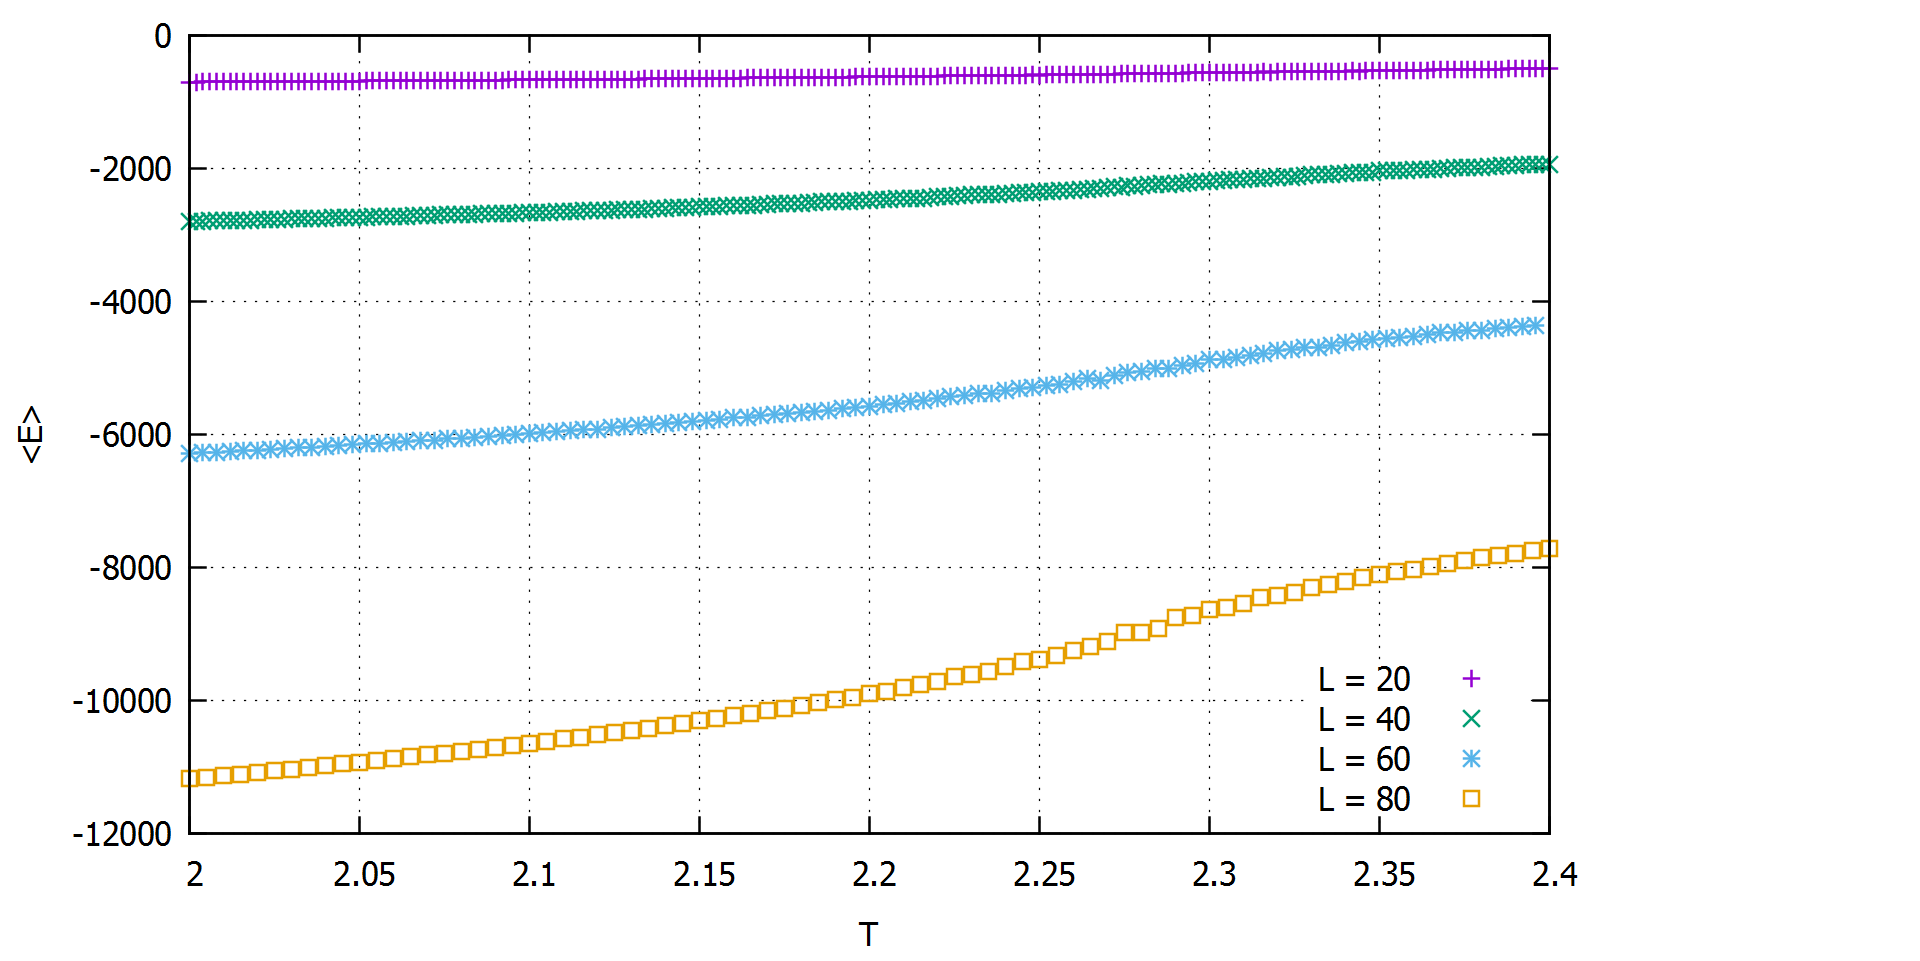
\includegraphics[scale = 0.25]{E_all.png}
	\centering
	\caption{Expectation value of the energy against temperature for different lattice sizes ($10^6$ Monte Carlo cycles)}
	\label{e_all}
\end{figure}

\begin{figure}[h]
	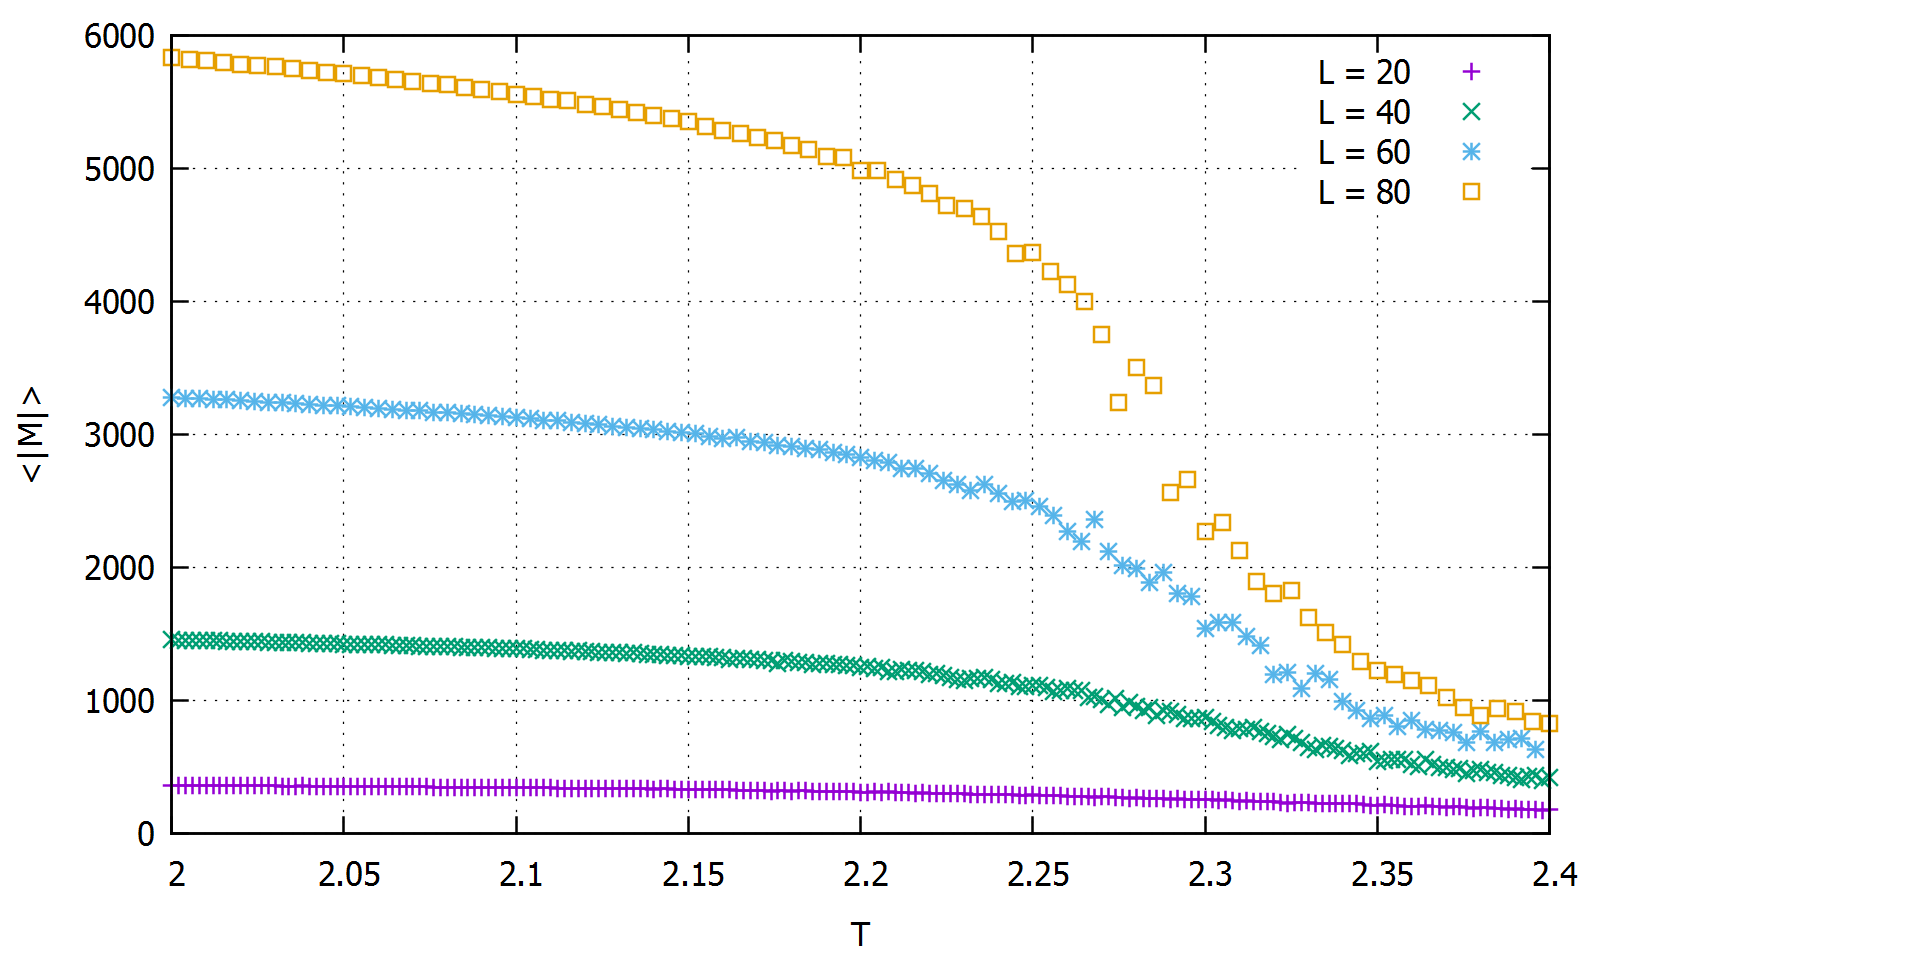
\includegraphics[scale = 0.25]{absm_all.png}
	\centering
	\caption{Expectation value of the absolute magnetisation against temperature for different lattice sizes ($10^6$ Monte Carlo cycles)}
	\label{absm_all}
\end{figure}

\begin{figure}[h]
	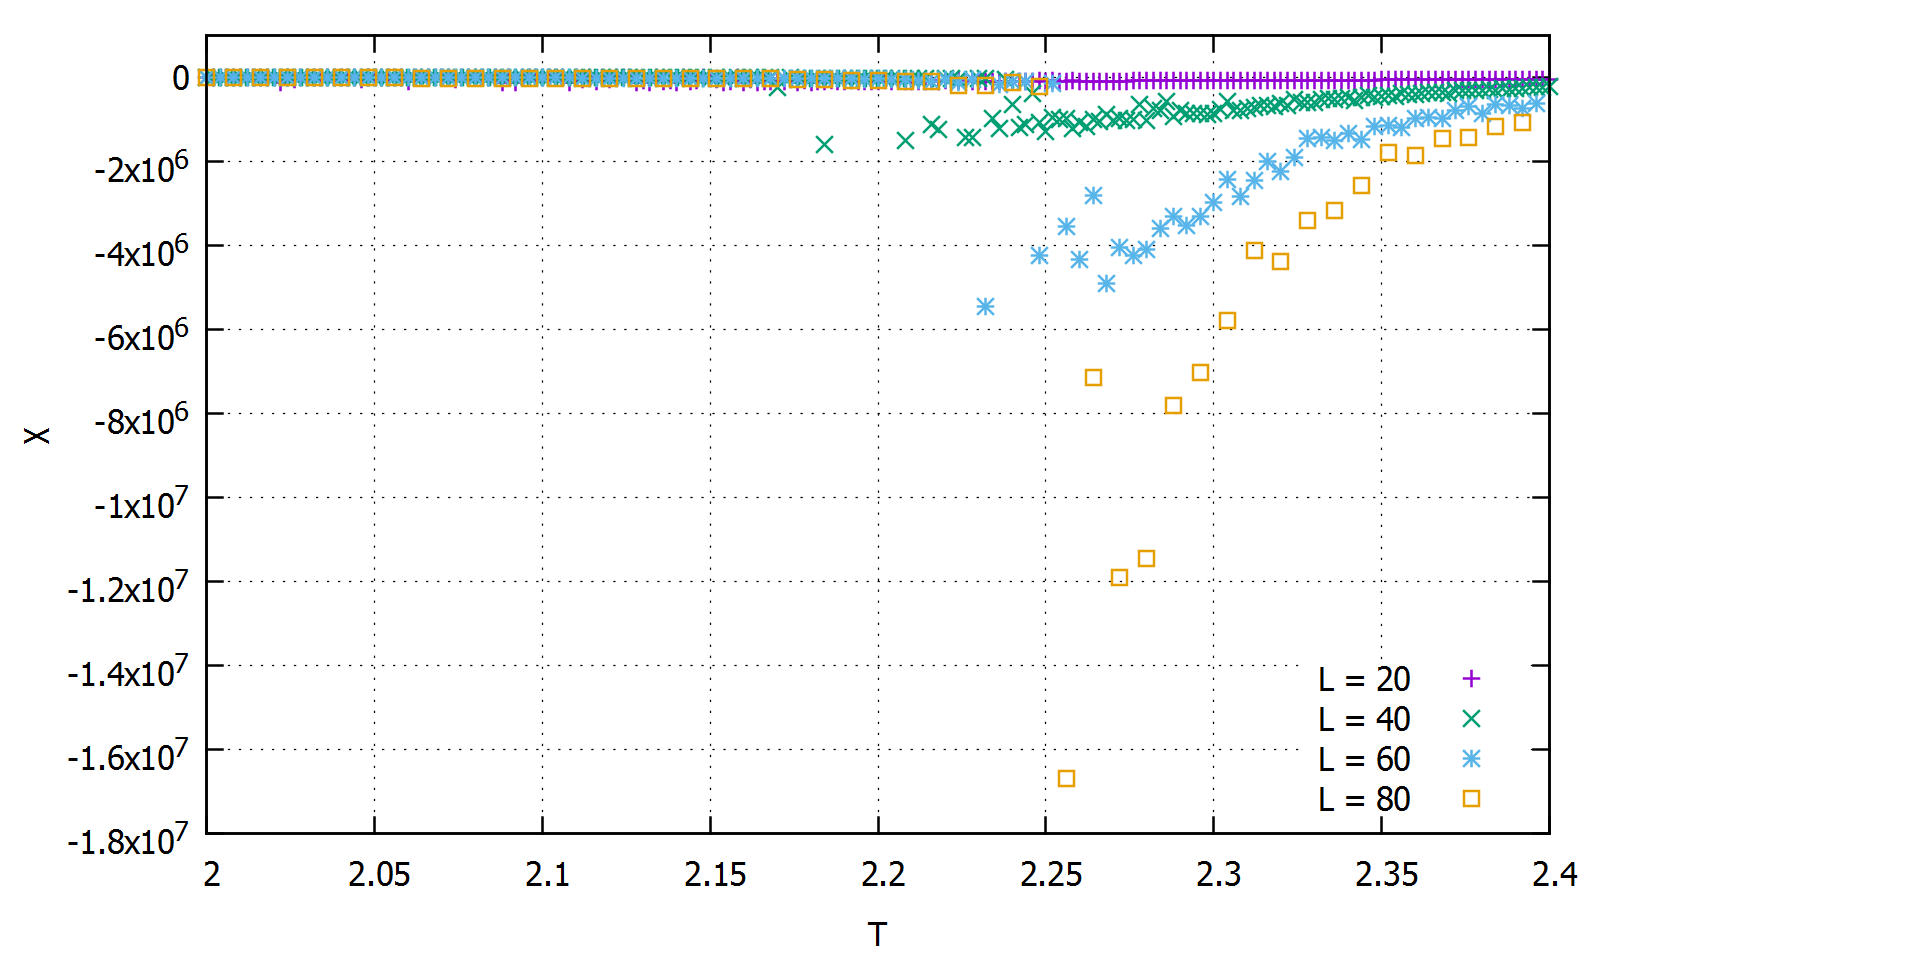
\includegraphics[scale = 0.25]{sus_all.png}
	\centering
	\caption{Susceptibility against temperature for different lattice sizes ($10^6$ Monte Carlo cycles)}
	\label{chi_all}
\end{figure}

\begin{figure}[h]
	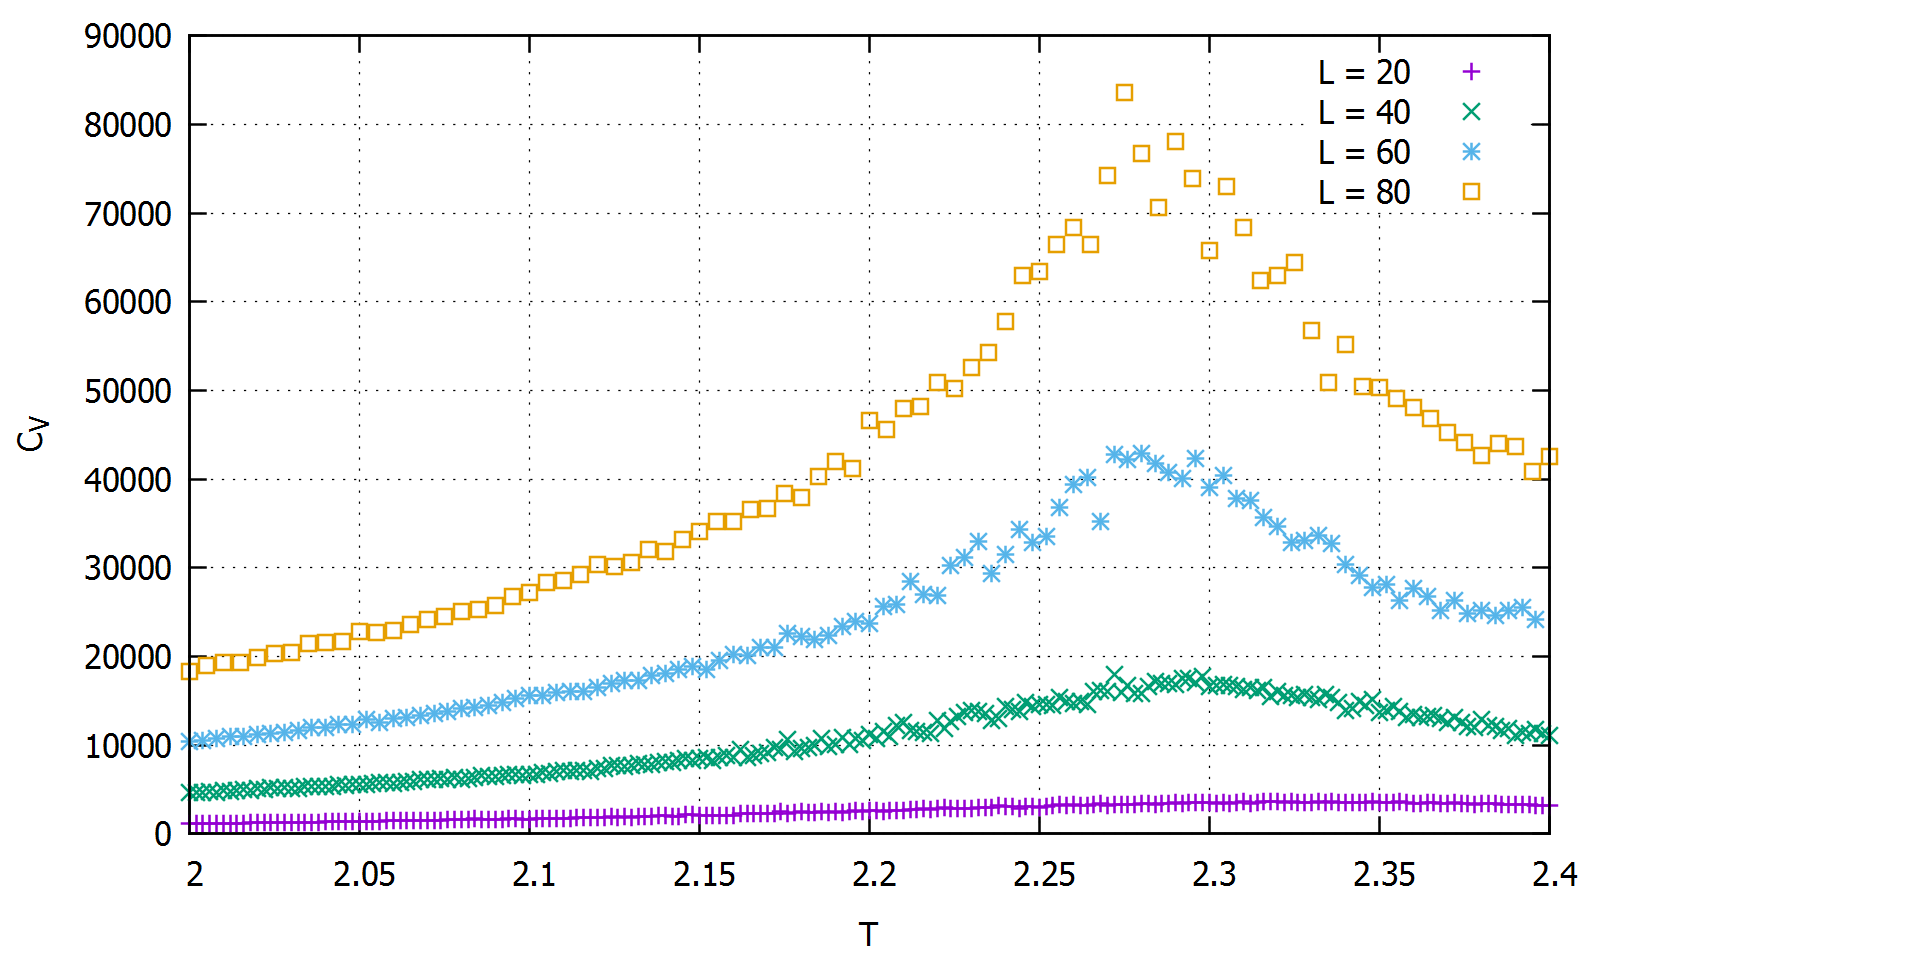
\includegraphics[scale = 0.25]{cv_all.png}
	\centering
	\caption{Expectation value of the specific heat against temperature for different lattice sizes ($10^6$ Monte Carlo cycles)}
	\label{cv_all}
\end{figure}

\begin{figure}[h]
	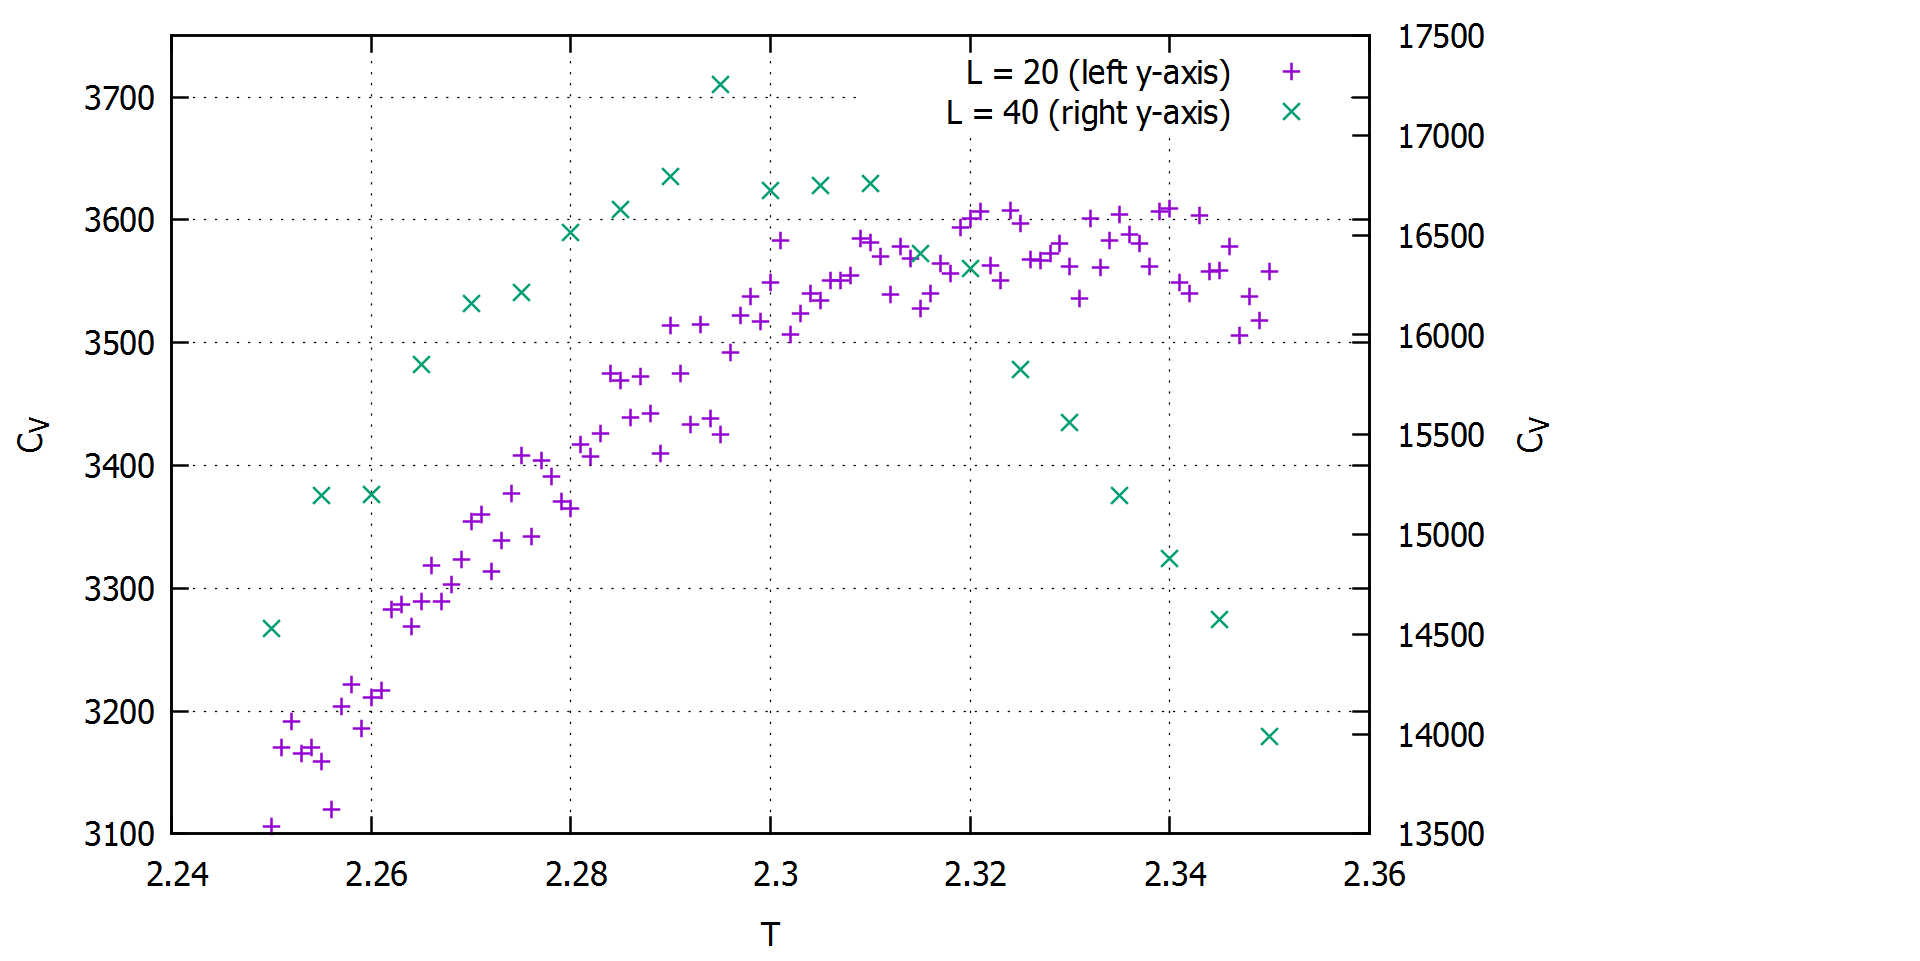
\includegraphics[scale = 0.25]{cv2040.png}
	\centering
	\caption{Expectation value of the specific heat against temperature for lattice sizes L = 20 and L = 40 ($5 \cdot 10^6$ Monte Carlo cycles)}
	\label{cv2040}
\end{figure}

\begin{figure}[h]
	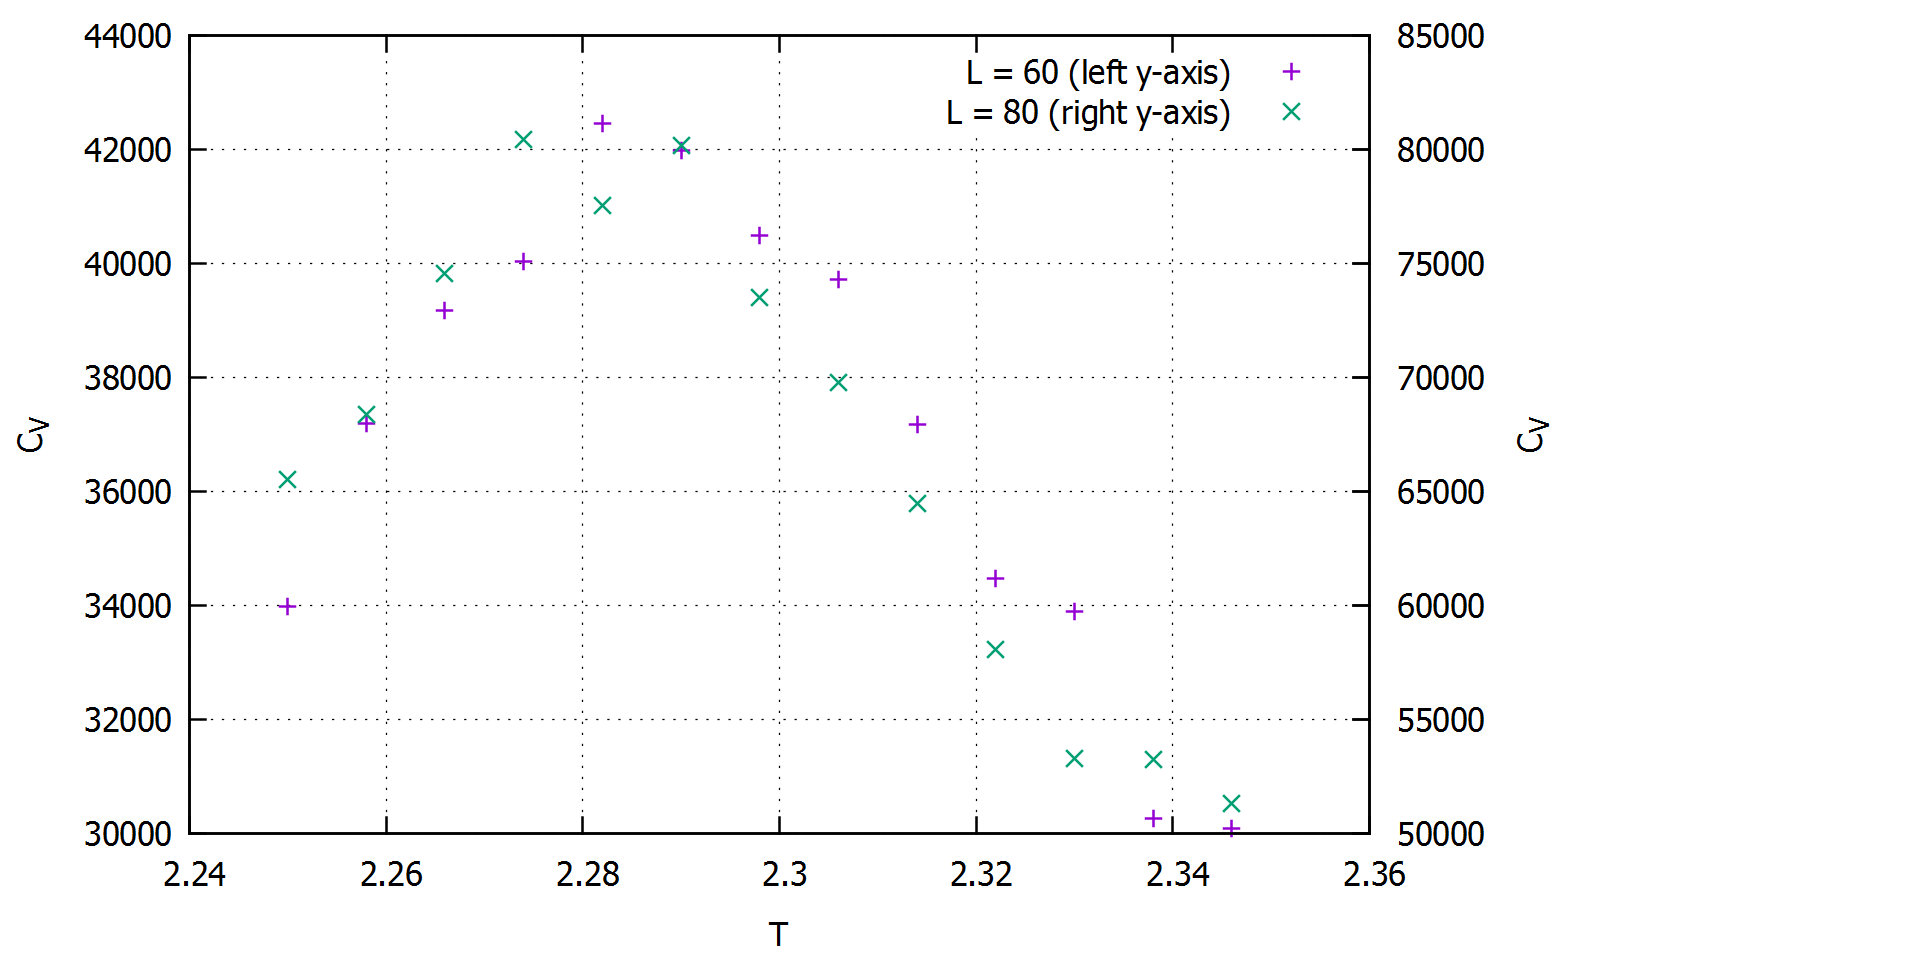
\includegraphics[scale = 0.25]{cv6080.png}
	\centering
	\caption{Expectation value of the specific heat against temperature for lattice sizes L = 60 and L = 80 ($5 \cdot 10^6$ Monte Carlo cycles)}
	\label{cv6080}
\end{figure}

\begin{table}[h!]
	\centering
	\begin{tabular}{|l|r|c|lrp{16cm}}\hline
		L & $T_C$ \\\hline
		20 & $(2.33 \pm 0.01)$\\
		40 & $(2.295 \pm 0.007)$\\
		60 & $(2.285 \pm 0.005)$\\
		80 & $(2.280 \pm 0.007)$\\\hline
	\end{tabular}
	\caption{Critical temperature for different lattice sizes L }
	\label{tc}
\end{table}

\begin{figure}[h]
	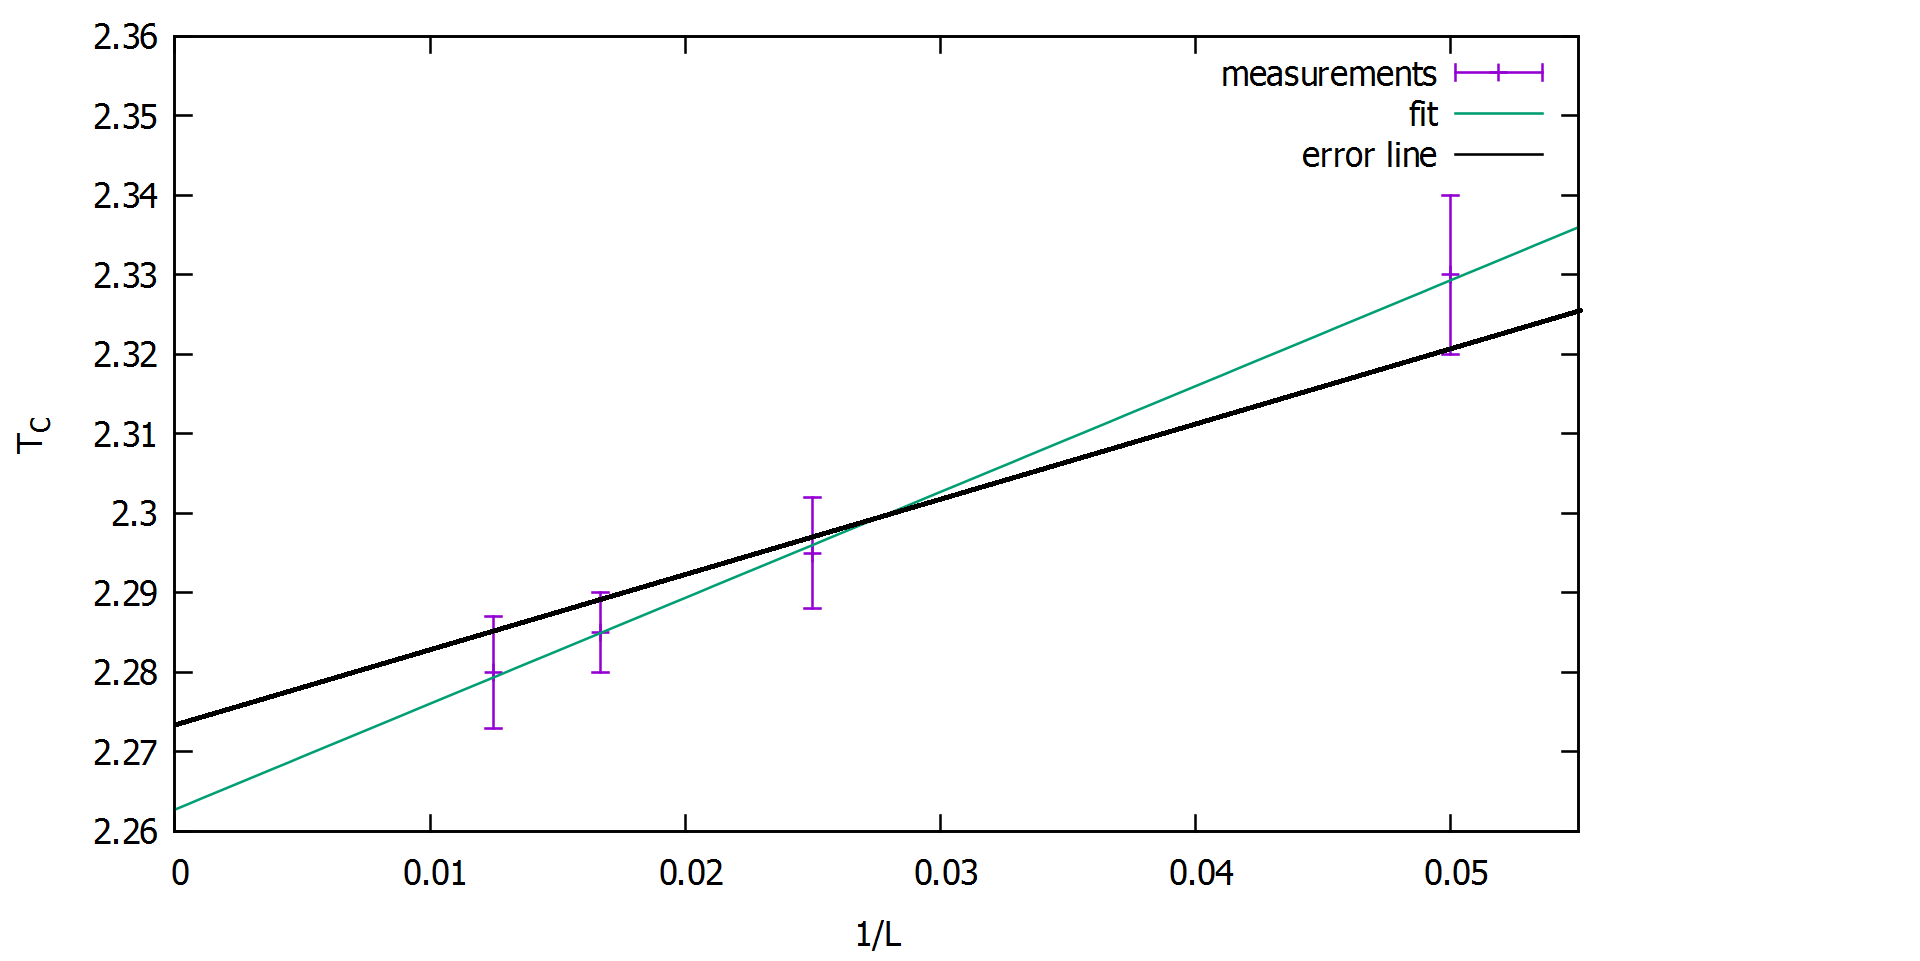
\includegraphics[scale = 0.25]{tc2.png}
	\centering
	\caption{Critical temperature $T_C$ against $\frac{1}{L}$}
	\label{tc2}
\end{figure}


% f part

The connection between different lattice sizes and the critical temperature is given by the following formula

\begin{equation}
T_C(L) - T_C(L = \infty) = a \cdot L^{-\frac{1}{\nu}}
\end{equation}

We have $\nu = 1$, so we get

\begin{equation}
T_C(L) = T_C(L = \infty) + a \cdot \frac{1}{L}
\end{equation}

If we now plot $T_C$ against $\frac{1}{L}$ we should get a line. By measuring the value at which the line crosses the y-axis we can determine $T_C(L = \infty)$. At figure \ref*{tc2} we have plotted our measured values for the critical temperature (which can be seen in table \ref*{tc}) against $\frac{1}{L}$ and signed in a fit line and an error line. The fit line crosses the y-axis at $T_C = 2.263$ while the error line crosses it at $T_C = 2.273$. Thus our value for the critical temperature for an infinite sized lattice is $T_C(L = \infty) = (2.26 \pm 0.01)$. The analytical solution $T_C^{a} = 2.269$ is in the first error interval of this value. Hence our value and the analytical solution match.



\subsection{Results}
As a first benchmark test for our program, we calculated the expectation values $<E>$, $<|M>|$, $<C_V>$ and $<\chi>$ of a $2\times2$-lattice for different temperatures. Those results could be easily compared to the analytical values from the part \ref{closed_solution}. In fig. \ref{b_E} -- \ref{b_chi}, you can see our results for these expectation values compared with the analytical solutions as functions of $T$. We took $10000$ Monte Carlo cycles for each temperature to achieve good results. You can see that the results fit very well to the analytical solutions which means that our program passed this benchmark test and works fine.

In the following table, we compared the analytical results for the different expectation values for a temperature $T=1.0$. It shows that all numerical results have a precision of at least two, in most cases of even three leading digits.
\begin{table}[h]
	\centering
	\caption{Analytical and numerical value of different expectaion values for $T=1.0$ in a $2\times2$-lattice}
	\begin{tabular}{ccc}
	& Analytical value & Numerical results \\\hline
	$<E>$ & $-7.983928$ & $-7.984080$ \\
	$<|M|>$ & $3.994642$ & $3.994760$ \\
	$<c_v>$ & $0.128329$ & $0.127107$ \\
	$<\chi>$ & $0.016043$ & $0.015494$	
	\end{tabular}	
\end{table}
\begin{figure}[h]
	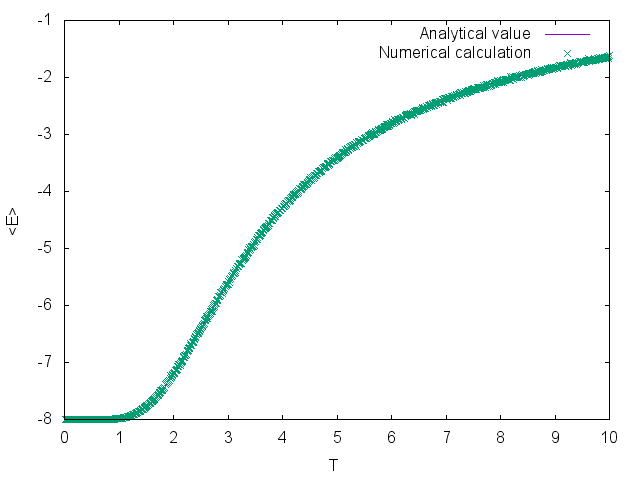
\includegraphics[width=\textwidth]{Energy.png}
	\caption{$<E>$ in a $2\times 2$-lattice for different temperatures\label{b_E}}
\end{figure}
\begin{figure}[h]
	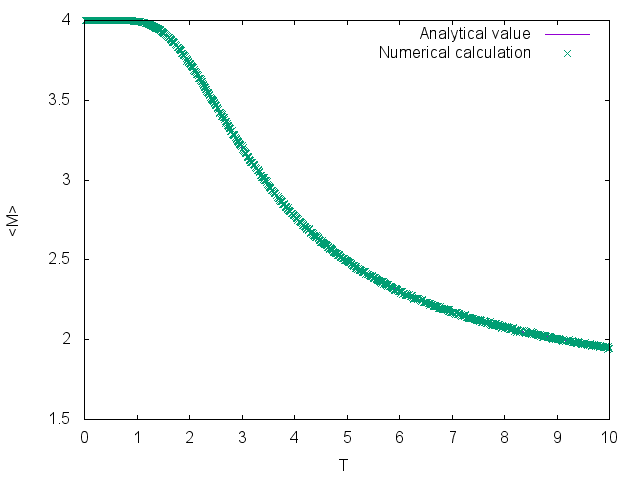
\includegraphics[width=\textwidth]{Magnetization.png}
	\caption{$<|M|>$ in a $2\times 2$-lattice for different temperatures\label{b_M}}
\end{figure}
\begin{figure}[h]
	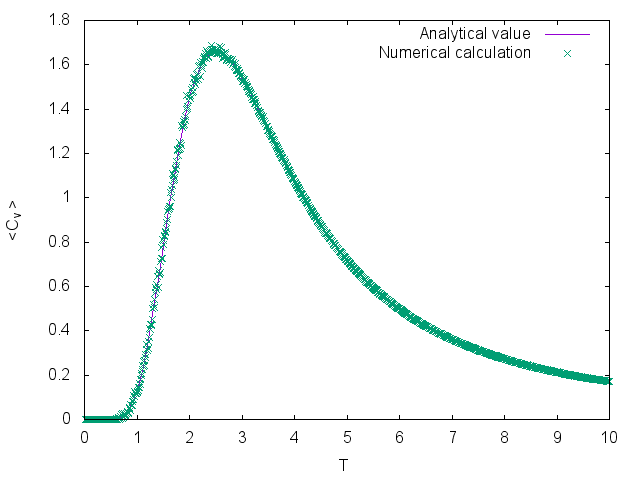
\includegraphics[width=\textwidth]{Heat_capacity.png}
	\caption{$<c_v>$ in a $2\times 2$-lattice for different temperatures\label{b_Cv}}
\end{figure}
\begin{figure}[h]
	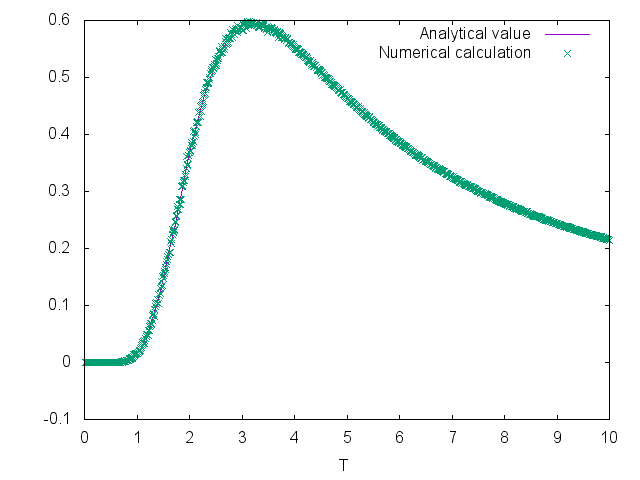
\includegraphics[width=\textwidth]{Susceptibility.png}
	\caption{$<\chi>$ in a $2\times 2$-lattice for different temperatures\label{b_chi}}
\end{figure}
In the next step, we took a closer look at the effect of thermalization. This term describes the process of the system slowly reaching the most likely state for a given temperature. When we start with a random setup, it is very unlikely that the system is already in this state at the beginning, but it will need some time (or, in our case, some Monte Carlo cycles) to reach it.

To get more insight in the process of thermalization, we observed the development of $<E>$ and $<|M|>$ of a $20\times20$-lattice for temperatures of $T=1.0$ and $T=2.4$, for both starting with a random setup and a lattice with all spins pointing in one direction. You can see that development in the figures \ref{c_1} -- \ref{c_4}, where these expectation values are plotted as function of the number of Monte Carlo cycles. We also plotted how many \glq moves\grq (flipping of spins) got accepted as a function of the number of cycles in fig. \ref{c_5} -- \ref{c_6} It is obvious that this value is proportional to the number of cycles and that, the higher the temperature is, the faster the number of accepted moves increases.

All these plots show that we need a bit more than $1000$ cycles in order to reach a stable state. This duration seems not to depend on the temperature, but obviously on the initial set-up: If this is close to a setup corresponding to the given temperature, it will not take long time to reach a stable state.

\label{results}
For later calculation, we set up a function called \emph{thermalization} for our program. This function performs the Metropolis algorithm without collecting data, instead it evaluates the energy after every 10 cycles. When the change between two measurements is less than $1\%$, the program starts collecting data. This takes in account the process described above and ensures that we reached a stable state before the actual calculations start.
\begin{figure}[h]
	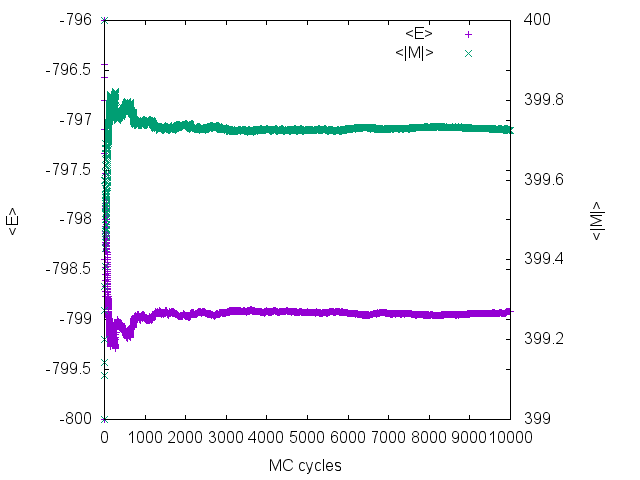
\includegraphics[width=\textwidth]{a1o.png}
	\caption{$<E>$ and $<|M|>$ in a $20\times 20$-lattice as a function of the number of Monte Carlo cycles, starting with ordered spins at $T=1.0$ \label{c_1}}
\end{figure}
\begin{figure}[h]
	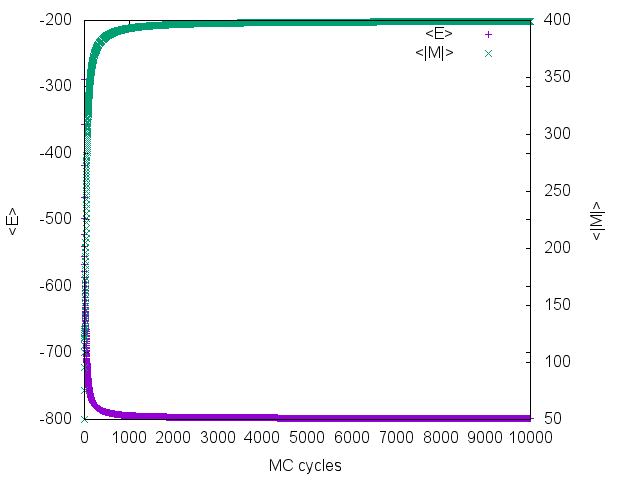
\includegraphics[width=\textwidth]{a1r.png}
	\caption{$<E>$ and $<|M|>$ in a $20\times 20$-lattice as a function of the number of Monte Carlo cycles, starting with random spins at $T=1.0$\label{c_2}}
\end{figure}
\begin{figure}[h]
	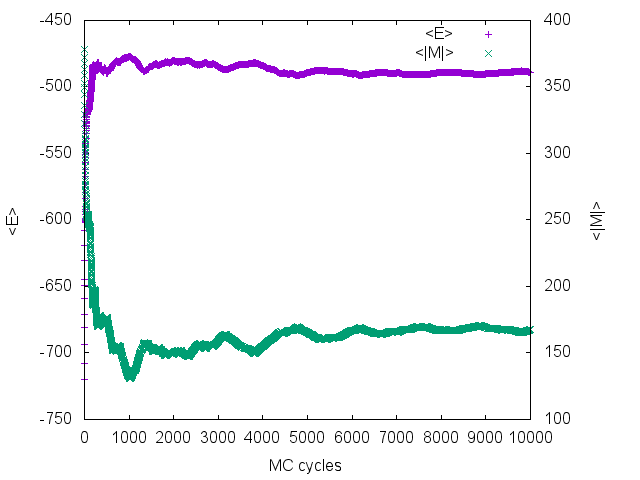
\includegraphics[width=\textwidth]{a24o.png}
	\caption{$<E>$ and $<|M|>$ in a $20\times 20$-lattice as a function of the number of Monte Carlo cycles, starting with ordered spins at $T=2.4$\label{c_3}}
\end{figure}
\begin{figure}[h]
	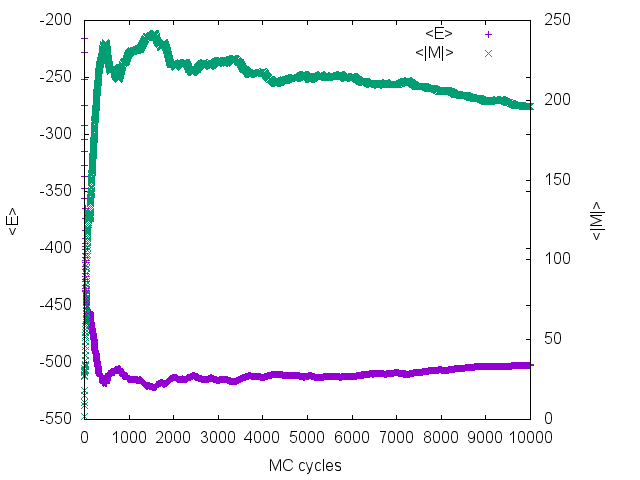
\includegraphics[width=\textwidth]{a24r.png}
	\caption{$<E>$ and $<|M|>$ in a $20\times 20$-lattice as a function of the number of Monte Carlo cycles, starting with random spins at $T=2.4$\label{c_4}}
\end{figure}

\begin{figure}[h]
	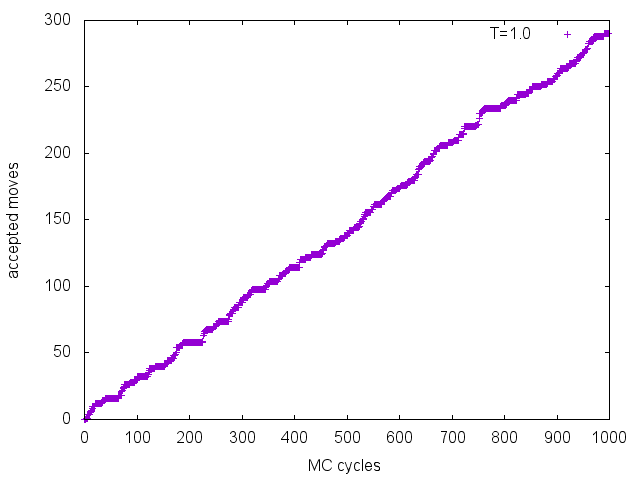
\includegraphics[width=\textwidth]{b1.png}
	\caption{The number of accepted spin flips as function of the number of cycles at $T=1.0$\label{c_5}}
\end{figure}
\begin{figure}[h]
	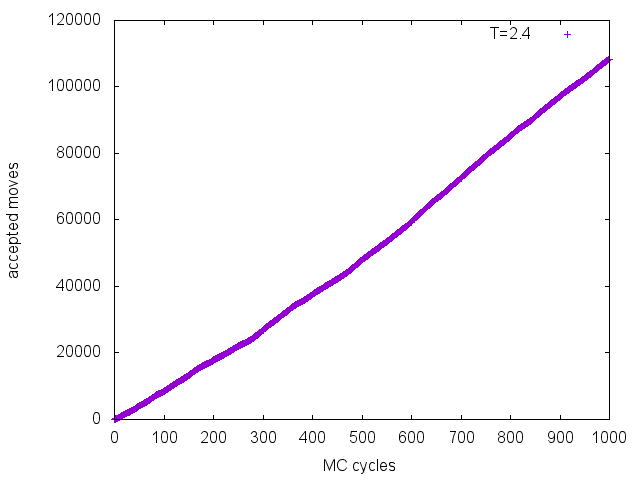
\includegraphics[width=\textwidth]{b24.png}
	\caption{The number of accepted spin flips as function of the number of cycles at $T=2.4$\label{c_6}}
\end{figure}

In the next step, we took a closer look at the probability of the single values of $E$ to appear. We observed a $2\times2$-lattice at a temperature of $T=1.0$ respectively $T=2.4$ again and did two histograms of how often an energy value occurred. Obviously, that distribution is expanded for a higher temperature. This correspondents with the fact that the variation of the energy for these temperatures is higher, which means that more values are accessed. Both histograms can be found in fig \ref{d1} -- \ref{d2}.

\begin{figure}[h]
	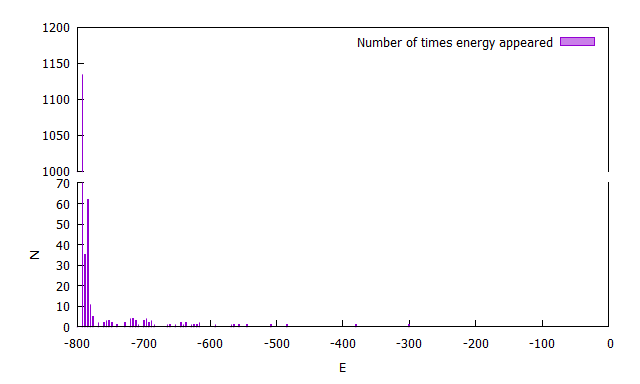
\includegraphics[width=\textwidth]{d1.png}
	\caption{Frequency of occurrence for different energies at $T=1.0$\label{d1}}
\end{figure}
\begin{figure}[h]
	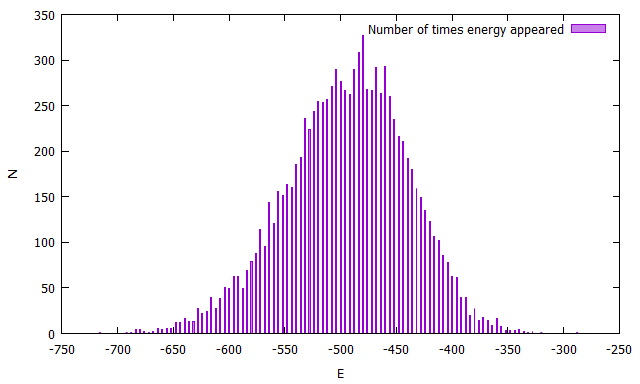
\includegraphics[width=\textwidth]{d24.png}
	\caption{Frequency of occurrence for different energies at $T=2.4$\label{d2}}
\end{figure}

\section{Comparison and discussion of results}

\section{source code}

\end{document}
